%% =====================================================================================
\section{Introduction}\label{sec:intro}
%% =====================================================================================

\subsection{Covering systems and the minimum modulus problem}

A \emph{covering system} is a finite collection of arithmetic progressions $a_1+d_1\Z,\dots,a_k+d_k\Z$ whose union
is $\Z$. It is \emph{distinct} if the moduli $d_1,\dots,d_k$ are pairwise distinct. For example,
\[
  0 \bmod 2,\quad 0 \bmod 3,\quad 1 \bmod 4,\quad 5 \bmod 6,\quad 7 \bmod 12
\]
is a distinct covering system with least modulus $2$. Covering systems were introduced by Erd\H{o}s in
1950~\cite{Erdos1950}, who asked whether there are distinct covering systems whose least modulus is arbitrarily
large; this is the \emph{minimum modulus problem}. Explicit constructions push the least modulus up to
$25$ (Gibson~\cite{Gibson2009}), $40$ (Nielsen~\cite{Nielsen2009}) and $42$ (Owens~\cite{Owens2014}), the largest
value known to occur.

In the other direction, Filaseta, Ford, Konyagin, Pomerance and Yu~\cite{FFKPY2007} showed that the sum of the
reciprocals of the moduli of a distinct covering system grows with its least modulus, and in 2015
Hough~\cite{Hough2015} resolved the minimum modulus problem negatively: every distinct covering system has least
modulus at most $10^{16}$. Balister, Bollob\'as, Morris, Sahasrabudhe and Tiba~\cite{BBMST} (henceforth BBMST)
introduced the \emph{distortion method}, which gives a simpler proof of Hough's theorem together with a much
better bound: congruences with distinct moduli, all at least $\prevBound$, do not cover $\Z$
\cite[Theorem~8.1]{BBMST}. The same method proves Schinzel's conjecture and gives lower bounds for the density of
the uncovered set \cite{BBMST}, and it has been used for related questions: the Erd\H{o}s--Selfridge problem for
squarefree moduli \cite{BBMST2021ES}; covering systems with squarefree moduli, where the least modulus is at most
$118$ \cite{CFT2025}; bounds for the $j$-th smallest modulus of a minimal covering system \cite{KKL2024} (see also
\cite{CFT2025}); covering systems whose reciprocal sums are close to $1$ \cite{FilasetaKalogirou2026}; and covering
systems of polynomial rings over finite fields, of global function fields and of number fields
\cite{LWWY2024,LWWY2025,BWang2026,LiWangYi2026}.

\subsection{The main results}

\begin{theorem}\label{thm:main}
Let $d_1,\dots,d_k$ be distinct integers, all at least $\Mzero$, and let $a_1,\dots,a_k\in\Z$. Then there is an
integer $x$ with $x\not\equiv a_i \pmod{d_i}$ for every $i$.
\end{theorem}

\begin{corollary}\label{cor:main}
Every covering system with distinct moduli has least modulus at most $\Mbound$. In particular, the largest least
modulus of a distinct covering system lies between $42$ and $\Mbound$.
\end{corollary}

The previous record was $\prevBound$ \cite{BBMST}. The proof of \cref{thm:main} is computer-assisted, in the limited
and precise sense explained in \cref{sec:intro-computer}. Its numerical part has been certified with outward rounding
and cross-checked by independently written code, and the new parts of the proof and of the computation have been
checked by an independent referee (an AI agent). Moreover, \cref{thm:main}, with the whole of its proof, has been
formally verified in Lean~4 with Mathlib, modulo one \texttt{native\_decide} evaluation of a numerical checker written
in Lean (\cref{sec:lean}). The formal proof evaluates the per-prime bounds in the same way, for the primes up to
$\XFormal$, and replaces the explicit prime-counting estimates behind \cite[Theorem~6.1]{BBMST} by a sharpened
elementary tail estimate (\cref{prop:tailtwo}). An earlier and independent formalization, with a simpler evaluation and
a checker of its own, verified the following weaker statement; its certificate is described in detail in
\cref{sec:certified-lean}.

\begin{theorem}\label{thm:lean}
Congruences with distinct moduli, all at least $\MzeroLean$, do not cover $\Z$. Hence every covering system with
distinct moduli has least modulus at most $\MboundLean$.
\end{theorem}

\subsection{Overview of the method}\label{sec:intro-overview}

Let $\cA$ be a finite family of progressions with distinct moduli, and let $p_1<p_2<\dots<p_n$ be the primes
dividing the lcm of the moduli. The distortion method of BBMST exposes the progressions prime by prime: at level
$i$ it removes the set $B_i$ covered by the progressions whose modulus has largest prime factor $p_i$. Writing
$\Z_{Q_i}=\Z_{Q_{i-1}}\times\Z/p_i^{\gamma_i}$, every point $x$ of $\Z_{Q_{i-1}}$ has a \emph{fibre}, and
$\alpha_i(x)$ denotes the proportion of the fibre covered by $B_i$. Starting from the uniform measure, BBMST build
probability measures $P_1,P_2,\dots$; the measure $P_i$ is obtained from $P_{i-1}$ by moving mass inside each fibre
from the covered to the uncovered points, but never multiplying the mass of a point by more than
$\nu_i=1/(1-\delta_i)$, where $\delta_i\in[0,1)$ is a parameter. The mass that stays on the covered points is the
\emph{loss}
\begin{equation}\label{eq:intro-loss}
  P_i(B_i)=\frac{\E_{P_{i-1}}\bigl[(\alpha_i-\delta_i)^+\bigr]}{1-\delta_i},
\end{equation}
and the progressions do not cover $\Z$ as soon as $\sum_i P_i(B_i)<1$.

BBMST bound the loss by the first and second moments of $\alpha_i$, using $(\alpha-\delta)^+\le\alpha^2/(4\delta)$,
the union bound $\alpha_i\le U$, where $U$ is a weighted count of the progressions through a point, and a bound
on the $P_{i-1}$-measure of a single progression. The quadratic majorant is exact only at $\alpha=2\delta$, and it
charges heavily covered fibres in proportion to $\alpha^2$.

Our main tool is a \emph{comparison theorem} (\cref{thm:comparison}). The distorted measure $P_{i-1}$ is a product
of conditional kernels, each bounded by $\nu_j$ times the uniform density. We show that for every measure of this
kind, every nonnegative combination $U$ of progressions and every convex nondecreasing $\varphi$,
\[
  \E_{P_{i-1}}[\varphi(U)]\le\E\bigl[\varphi(U^{\mathrm{al}})\bigr],
\]
where $U^{\mathrm{al}}$ is obtained by moving all progressions so that they pass through one point, and by
evaluating the resulting count at a random point whose $p_j$-adic valuations $V_j$ are independent with the
\emph{tilted} law $\P(V_j\ge a)=\min(1,\nu_j p_j^{-a})$. Alignment maximizes the overlap of the progressions; for
the uniform measure and $\varphi(u)=(u-1)^+$ the statement is Rogers' theorem on sieving
(\cref{sec:rogers}).

We apply the comparison theorem to the hinge $\varphi(u)=(u-t)^+$ with $0\le t\le\delta_i$. Together with a pointwise
inequality (\cref{lem:pointwise}) and an enlargement of the family to all admissible moduli, which is where the
distinctness of the moduli enters (\cref{lem:enlargement}), it gives the bound (\cref{thm:perprime})
\begin{equation}\label{eq:intro-perprime}
  P_i(B_i)\le\frac{\E\bigl[(U_p(s)-t)^+\bigr]}{1-t},\qquad U_p(s)=\sum_{d\mid s}w_p(d),\qquad
  w_p(d)=\sum_{j\ge1:\,dp^j\ge m}p^{-j},
\end{equation}
where $p=p_i$, $m$ is the least modulus, and $s=\prod_{q<p}q^{v_q}$ is a random $(p-1)$-smooth number with
independent exponents, $\P(v_q\ge a)=\min(1,\nu_q q^{-a})$. The right-hand side depends only on $m$, $p$ and the
parameters $\delta_q$, not on the progressions.

It remains to show that, for $m=\Mzero$ and a suitable choice of the $\delta_q$, the sum over all primes of the
right-hand side of \eqref{eq:intro-perprime} is less than $1$. For every prime $p\le\PmaxMain$ we evaluate it
exactly, up to truncations whose effect is bounded explicitly (\cref{sec:evaluation}): for $p<m/2$ by an identity
that splits the primes below $p$ into three ranges and reduces the expectation to an enumeration and a
two-dimensional law, and for $p>m/2$ by a factorization of the divisor count of $s$. A certified program with
directed rounding shows that the total for $p\le\PmaxMain$ is at most $\etaMain$, and a criterion of BBMST handles
the larger primes (\cref{sec:computation}). The formal proof uses the same evaluation for $p\le\XFormal$ together
with an elementary tail estimate; for $m=\MzeroLean$ a cruder evaluation suffices, and that version was formalized
first. \Cref{fig:cumulative} shows the running
totals. With the distortion parameters of the certificate for $m=\MzeroLean$, the moment bounds of BBMST would
exhaust the whole budget at $p=\bbPassP$.

\subsection{What is new}\label{sec:intro-new}

The comparison theorem extends a classical inequality, and we are careful about what is prior art.
\begin{itemize}
\item \emph{Rogers' theorem} \cite[pp.~242--244]{HalberstamRoth1966} states that, for fixed moduli, the density of
  the integers avoiding the progressions is largest when all the residues are equal. It was proved independently by
  Simpson \cite[Lemma~2.3]{Simpson1986} and was revisited by Tao \cite{TaoRogers2026}, whose compression argument
  has the same structure as our one-coordinate lemma plus induction. Lewis \cite{Lewis1996} and Filaseta et al.
  \cite{FFKPY2007} cite it. It is the case $\nu\equiv1$, unit weights and $\varphi(u)=(u-1)^+$ of
  \cref{thm:comparison}.
\item \emph{Filaseta and Kalogirou} \cite{FilasetaKalogirou2026} used Rogers' theorem (via Lewis) in the
  undistorted stages ($\delta=0$) of a distortion argument, together with the fourth-moment bound
  $(\alpha-\delta)^+\le 27\alpha^4/(256\,\delta^3)$ for the loss. This is prior art for the fractional-moment bounds
  of \cref{sec:theta}.
\item \emph{BBMST's moment lemma} \cite[Lemma~3.6]{BBMST} is the monomial case $\varphi(u)=u^k$ of
  \cref{thm:comparison}, and \cite[Lemma~3.4]{BBMST} is its single-progression case (\cref{sec:bbmst-lemmas}).
\end{itemize}
What is new is the extension in two directions at once: to measures given by $\nu$-bounded product kernels, which
is what makes the inequality applicable to the distorted measures and produces the tilted law; and to the whole
increasing convex order, which allows the non-polynomial hinge $(u-t)^+$. We found no earlier use of convex-order
or tilted comparison inequalities to bound the distortion losses themselves. Two further, minor novelties are the
exact evaluation of the per-prime bounds (\cref{lem:SBH,lem:tausplit}), which is elementary, and an elementary tail
estimate (\cref{prop:tail,prop:tailtwo}) based on Chebyshev's bound for the central binomial coefficient, which can replace
\cite[Theorem~6.1]{BBMST} and Dusart's estimate for the $k$-th prime when the margin is not too small.

\subsection{What is computer-assisted, and what has been checked}\label{sec:intro-computer}

\Cref{thm:criterion} and \cref{prop:bbmst61} reduce \cref{thm:main,thm:lean} to finitely many inequalities between
explicit numbers: the sum over the primes $p\le P_{\max}$ of upper bounds $c_p$ for the expectations in
\eqref{eq:intro-perprime}, together with a term for the larger primes, must be less than $1$. The computer evaluates
these finitely many quantities (for $\kPrimesMain$ primes in the case of \cref{thm:main}) in IEEE double precision
with directed rounding, so that the printed totals are rigorous upper bounds (\cref{sec:rounding}). No search over
covering systems is involved. The distortion parameters were found by floating-point searches, but they are simply
inputs: any choice in $[0,\tfrac12]$ gives a valid bound.

The certificate for \cref{thm:main} has been cross-checked by independently written code, with no violation at any
prime (\cref{sec:xcheck}). An independent referee (an AI agent) checked the new evaluation by hand and by brute force,
audited the rounding and the truncations, and recomputed every per-prime bound up to $\PmaxMain$ with separately
written programs; it found the sum of the exact bounds to lie in $[\refEtaLo,\refEtaHi]$ and found no errors. The
proofs of \cref{thm:main,thm:lean}, each including a separate numerical checker written in Lean, have been formally
verified (\cref{sec:lean}): the only step that is not checked by Lean's kernel is the compiled evaluation of the
checker, which takes about ten minutes for \cref{thm:main}. The certificate for \cref{thm:lean} has also been
reproduced by independent code. \Cref{tab:status} summarizes the status of all results of this paper.

\begin{table}[ht]
\centering
\caption{The results of this paper and how they have been checked. ``Certified'': a computation with outward
rounding; ``cross-checked'': recomputed by independently written code; ``refereed'': checked by an independent AI
agent. No result has yet been refereed by human experts.}
\label{tab:status}
\small
\begin{tabular}{@{}l>{\raggedright\arraybackslash}p{0.38\textwidth}>{\raggedright\arraybackslash}p{0.46\textwidth}@{}}
\toprule
theorem & statement & status\\
\midrule
\ref{thm:main} & least modulus $\le\Mbound$ & certified, cross-checked, refereed; formally verified in Lean~4 (one
  \texttt{native\_decide})\\
\ref{thm:lean} & least modulus $\le\MboundLean$ & certified, cross-checked; formally verified in Lean~4 (one
  \texttt{native\_decide}; an earlier, independent formalization with its own checker)\\
\ref{thm:squarefree} & squarefree moduli: least modulus $\le7$ & certified, recomputed, formally verified in Lean~4
  (one \texttt{native\_decide})\\
\ref{thm:sf23} & squarefree, $23$-smooth moduli $\ge3$ never cover & certified, recomputed exactly by independent
  code, refereed; formally verified in Lean~4 (one \texttt{native\_decide})\\
\ref{thm:sf29} & squarefree, $29$-smooth moduli $\ge3$ never cover & certified, recomputed exactly by independent
  code, refereed; not formalized\\
\ref{thm:sf7type} & squarefree moduli: least modulus $\le6$ (moduli $\ge7$ never cover) & certified,
  recomputed exactly by independent code, refereed; formally verified in Lean~4 ($124$ \texttt{native\_decide}
  evaluations)\\
\ref{thm:sf6smooth} & squarefree, $211$-smooth moduli $\ge6$ never cover & certified, recomputed exactly by
  independent code, refereed; not formalized\\
\ref{thm:odd} & odd moduli: divisibility conditions (A)--(C) & certified, refereed; formally verified in Lean~4 (one
  \texttt{native\_decide} each)\\
\ref{thm:odd2} & six further divisibility conditions & certified, refereed; formally verified in Lean~4 (one
  \texttt{native\_decide} each)\\
\ref{thm:rings} & $\mathbb{F}_q[x]$, genus-$0$ function fields, $\Z[i]$, $\Z[\omega]$ & certified, refereed with
  independent checkers; not formalized\\
\bottomrule
\end{tabular}
\end{table}

\subsection{Organization}

\Cref{sec:distortion} recalls the distortion method. \Cref{sec:comparison} states and proves the comparison theorem
and relates it to Rogers' theorem and to the lemmas of BBMST. \Cref{sec:loss} derives the bound on the loss at one
prime and reduces the theorems to a finite computation. \Cref{sec:evaluation} explains how the bound is evaluated,
and \cref{sec:computation} describes the certified computations, their independent verification and the
formalization. \Cref{sec:limits} discusses which steps of the method are sharp and where the remaining slack lies.
\Cref{sec:further} describes applications to squarefree and odd moduli and to other rings. The appendices list the
distortion schedules, the budgets by prime ranges, the rounding conventions of the checkers and instructions for
reproducing the computations.

\begin{figure}[t]
  \centering
  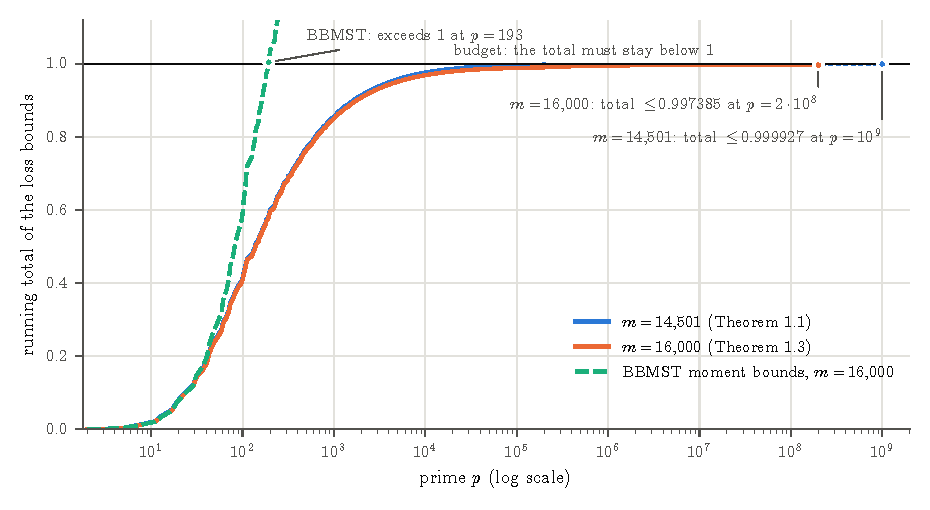
\includegraphics[width=\textwidth]{fig/cumulative_loss.pdf}
  \caption{Running totals of the certified per-prime loss bounds $c_p$ for the certificates of \cref{thm:main}
  ($m=\Mzero$, blue) and of \cref{thm:lean} ($m=\MzeroLean$, orange), for all primes up to $\PX$; beyond, the orange
  curve shows every $20{,}000$-th prime, and the dotted blue segment joins the value at $\PX$ to the certified total
  at $p=\PmaxMain$. The criterion needs the total to stay below $1$. The dashed curve shows the moment bounds
  $b_p=\min\bigl(\E[U_p],\,\E[U_p^2]/(4\delta_p(1-\delta_p))\bigr)$ of BBMST at $m=\MzeroLean$, computed from the
  same certified first and second moments and with the same distortion parameters; their total exceeds $1$ at
  $p=\bbPassP$ and reaches about $2.2$ at $p=\PX$.}
  \label{fig:cumulative}
\end{figure}
% CHECK: logs/xcheck_final.md says the BBMST-type total "reaches 2.19 by 2e5"; recomputing it from
%        logs/dump16k.txt (make_figures.py) gives 2.1849.  The text says "about 2.2", which covers both.
